\subsubsection{Scopo}
Lo scopo di questo processo consiste nell'illustrazione di come deve essere redatta e mantenuta
la documentazione, durante il \gl{ciclo di vita} del \gl{software}.
\subsubsection{Aspettative}
Le aspettative della corretta implementazione di tale processo sono:
\begin{itemize}
	\item una chiara visione della documentazione prodotta durante il \gl{ciclo di vita}
del \gl{software};
	\item una serie di norme per la stesura di documenti coerenti e validi;
	\item una documentazione formale e coerente.
\end{itemize}
\subsubsection{Descrizione}
In questo documento devono essere redatte tutte le norme e le convenzioni adottate dal gruppo,
in modo da produrre una documentazione valida e coerente.
\subsubsection{Procedure}
Per la stesura della documentazione si è utilizzato il linguaggio \LaTeX{}, si veda la \hyperref[sec:Strumenti]{sezione strumenti \ref*{sec:Strumenti}}.
 \paragraph{Approvazione dei documenti}
La formalizzazione di un documento segue la seguente procedura:
\begin{enumerate}
	\item il documento viene redatto da coloro che sono incaricati della sua stesura ed eventuale correzione di errori;
	\item per ogni significativa modifica del documento, i \VERP{} avranno il compito di controllare la presenza di errori o imprecisioni;
	\item se i \VERP{} riscontrano degli errori, dovranno notificarlo ai redattori del documento tramite una specifica \gl{issue}, tornando così al punto 1, altrimenti, se completo, il documento viene consegnato al \RESP{};
	\item il \RESP{} di \gl{progetto} decide se approvare, e quindi formalizzare il documento, oppure se rifiutarlo comunicando la motivazione e le modifiche da apportare, tornando così al punto 1.
\end{enumerate}
\begin{figure}[h]
\centering
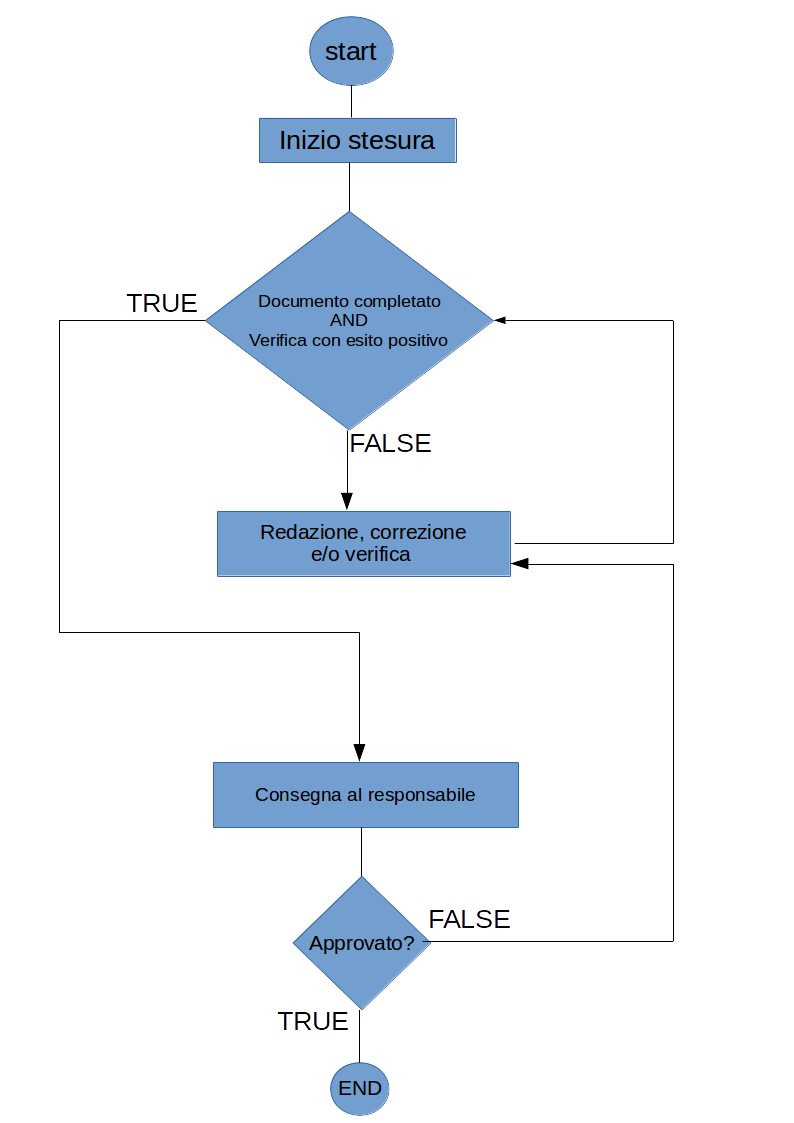
\includegraphics[scale=0.4]{img/flussoapprovazione.png}
\caption{Flow chart dell'approvazione di un documento}\label{sec:Figura2}
\end{figure}
\subsubsection{Template}
Per garantire omogeneità tra i documenti è stato creato un \gl{template} \LaTeX{}, dove sono state definite tutte le regole di formattazione da applicare al documento. Questo permette a tutti i componenti del gruppo di concentrarsi solo nella stesura del contenuto, senza doversi preoccupare dell'aspetto. 
\subsubsection{Struttura dei documenti}
 \paragraph{Frontespizio} 
La prima pagina di ogni documento dovrà contenere:
\begin{itemize}
	\item logo del gruppo;
	\item nome del \gl{progetto};
	\item nome del documento e la relativa versione;
	\item sommario;
	\item data di redazione;
	\item nome e cognome dei redattori del documento;
	\item nome e cognome dei verificatori del documento;
	\item nome e cognome del responsabile per l'approvazione del documento;
	\item uso del documento (interno o esterno);
	\item lista di distribuzione del documento.
\end{itemize}
 \paragraph{Diario delle modifiche}
 La seconda pagina dovrà contenere il diario delle modifiche di quel determinato documento.\\
 Il diario è costituito di una tabella ordinata in modo decrescente seconda la data di modifica e il numero di versione.\\
 Gli attributi della tabella rappresentano:
 \begin{itemize}
 	\item numero di versione;
 	\item breve riepilogo delle modifiche apportate;
 	\item autore delle modifiche;
 	\item ruolo ricoperto dall'autore all'interno del \gl{progetto};
 	\item data di modifica.
 \end{itemize}
 \paragraph{Indice}
 In ogni documento è presente un indice delle sezioni, utile a fornire una visione macroscopica della struttura del documento. Sono previsti, se necessari, gli indici relativi alle tabelle e alle figure presenti nel documento in questo ordine.
 \paragraph{Intestazione e piè di pagina}
L'intestazione delle pagine di ogni documento deve contenere:
\begin{itemize}
	\item numero e titolo della sezione;
	\item nome del \gl{progetto}.
\end{itemize} 
Il piè di pagina contiene invece:
\begin{itemize}
	\item nome del documento con la relativa versione;
	\item nome del gruppo;
	\item pagina X di Y, dove X è la pagina corrente e Y è il numero di pagine totali del documento.
\end{itemize} 
\subsubsection{Versionamento}
Ciascun documento che verrà redatto dovrà essere versionato, per consentire un tracciamento chiaro della sua storia e delle sue modifiche.\\Verrà applicato il seguente formalismo:\\ \\ \centerline{vX.Y.Z}\\ \\dove:
\begin{itemize}
	\item \textbf{X}:
	\begin{itemize}
		\item inizia da 0;
		\item viene incrementato quando il \RESP{} di \gl{progetto} approva il documento.
	\end{itemize}
	\item \textbf{Y}:
	\begin{itemize}
		\item inizia da 0;
		\item viene incrementato dal \VER{} ad ogni \gl{verifica};
		\item quando viene modificato X, viene riportato a 0.
	\end{itemize}
	\item \textbf{Z}:
	\begin{itemize}
		\item inizia da 0;
		\item viene incrementato dal Redattore del documento dopo ogni modifica;
		\item quando viene modificato Y, viene riportato a 0.
	\end{itemize}
\end{itemize}
\subsubsection{Norme tipografiche}
In questa sezione vengono definite le norme ortografiche e tipografiche da rispettare nella stesura di ogni documento.
 \paragraph{Stile del testo} 
\begin{itemize}
	\item \textbf{Grassetto}: viene utilizzato per:
	\begin{itemize}
		\item titoli;
		\item elementi di un elenco puntato che riassumono il contenuto del relativo paragrafo.
	\end{itemize}
	\item \textbf{Corsivo}: viene utilizzato per:
	\begin{itemize}
		\item citazioni;
		\item abbreviazioni;
		\item parole inserite nel glossario;
		\item riferimenti ad altri documenti;
		\item nomi di società o aziende;
		\item ruoli dei membri del gruppo.
	\end{itemize}
	\item \textbf{Maiuscolo}: le parole scritte interamente in maiuscolo dovranno riferirsi soltanto ad acronimi.
	\item \textbf{Monospace}: le porzioni di testo scritte in monospace definiscono:
	\begin{itemize}
		\item frammenti di codice;
		\item comandi;
		\item URL.
	\end{itemize}
	\item \textbf{Glossario}: le parole che hanno un riferimento nel glossario sono in corsivo e hanno una 'g' a pedice.
\end{itemize}
 \paragraph{Elenchi puntati}
Tutti gli elenchi puntati sono caratterizzati graficamente da un pallino nel primo livello, da una trattino nel secondo e da un asterisco nel terzo (automatizzato grazie al \gl{template} \LaTeX{}{} creato). \\
Ogni elemento deve terminare con il punto e virgola, a meno che non sia l'ultimo dell'elenco, in questo caso la frase va terminata con il punto. Ogni punto inizia con la minuscola, tranne nel caso in cui necessiti di una spiegazione: allora
si utilizzerà la maiuscola.
 \paragraph{Formati comuni}
\begin{itemize}
	\item \textbf{Date}:\\ \\ \centerline{AAAA - MM - GG} \\ \\
	dove:
	\begin{itemize}
		\item AAAA: rappresenta l'anno utilizzando 4 cifre;
		\item MM: rappresenta il mese utilizzando 2 cifre;
		\item GG: rappresenta il giorno utilizzando 2 cifre.
	\end{itemize}
	\item \textbf{Orari}:\\ \\ \centerline{HH:MM} \\ \\dove:
	\begin{itemize}
		\item HH: rappresenta l'ora e può assumere valori da 0 a 23;
		\item MM: rappresenta i minuti e può assumere valori da 0 a 59.
	\end{itemize}
	\item \textbf{Nomi ricorrenti}:
	\begin{itemize}
		\item \textbf{Ruoli di \gl{progetto}}: ogni nome di un ruolo di \gl{progetto} deve essere scritto con la lettera iniziale maiuscola e con lo stile corsivo. Questo viene automatizzato utilizzando il comando "\textbackslash{CodiceRuolo}";
		\item \textbf{Nomi propri}: ogni nome deve essere espresso nella forma "Nome Cognome";
		\item \textbf{Nomi dei documenti}: ogni nome di documento viene scritto con lo stile corsivo, con l'iniziale di ogni parola maiuscola e con la versione corrente. Questo viene automatizzato richiamando il comando "\textbackslash{SiglaDocumentodoc}".
	\end{itemize}
\end{itemize}
 \paragraph{Sigle}
E' previsto l'utilizzo di queste sigle:
\begin{itemize}
	\item \textbf{AdR}: per \ARdoc;
	\item \textbf{PdP}: per \PPdoc;
	\item \textbf{NdP}: per \NPdoc;
	\item \textbf{SdF}: per \SFdoc;
	\item \textbf{PdQ}: per \PQdoc;
	\item \textbf{ST}: per \STdoc;
	\item \textbf{Gl}: per \Gldoc;
	\item \textbf{DP}: per \DPdoc.		
\end{itemize}
 
\subsubsection{Elementi grafici}
 \paragraph{Tabelle} 
 Le tabelle devono essere accompagnate da una didascalia e da un numero incrementale per
garantirne la tracciabilità.
 \paragraph{Immagini}
Ogni immagine deve essere centrata orizzontalmente. Inoltre deve
essere nettamente separata dai paragrafi che la seguono e la precedono, in modo da definire un netto distacco tra testo e grafica e migliorare conseguentemente la leggibilità. Essa dev'essere accompagnata da una didascalia analoga a quella descritta per le tabelle. Tutti i diagrammi
\gl{UML} vengono inseriti nel documento sotto forma di immagine.
\subsubsection{Classificazione dei documenti}
 \paragraph{Documenti informali}
 Tutti i documenti sono da ritenersi informali fino all'approvazione da parte del \RESP{} di \gl{progetto}, ed in quanto tali sono da considerarsi esclusivamente ad uso interno.
 \paragraph{Documenti formali}
 Un documento viene definito formale quando viene validato dal \RESP{} di \gl{progetto}. Solo i documenti formali possono essere distribuiti all'esterno del gruppo. Per arrivare a tale stato il
documento deve aver passato la \gl{verifica} e la \gl{validazione}.
 \paragraph{Glossario}
Il glossario nasce dall'esigenza di chiarire il significato di parole che possono risultare ambigue all'interno di determinati contesti. Saranno quindi presenti parole che:
\begin{itemize}
	\item trattano argomenti tecnici;
	\item possono creare delle ambiguità sul significato;
	\item rappresentano delle sigle.
\end{itemize}
La struttura deve avere queste caratteristiche:
\begin{itemize}
	\item le parole devono essere in ordine alfabetico;
	\item ogni termine deve essere seguito da una spiegazione chiara e concisa, che non generi alcun tipo di ambiguità.
\end{itemize}
 \paragraph{Verbali}
Questo documento ha lo scopo di riassumere in modo formale le discussioni effettuate e le decisioni prese durante le riunioni. I verbali, come le riunioni, sono classificati in: interni ed esterni. In
particolare i verbali esterni, essendo documenti ufficiali, devono essere redatti dal \RESP{} di Progetto.
Ogni verbale dovrà essere denominato nel seguente modo:\\ \\
\centerline{\textit{Verbale\textunderscore{TipoVerbale}\textunderscore{DataVerbale}}}
\\ \\
dove:
\begin{itemize}
	\item \textbf{TipoVerbale}: identifica se il verbale è riferito ad una riunione interna (I) o esterna (E);
	\item \textbf{DataVerbale}: identifica la data nella quale si è svolta la riunione relativa al verbale.
\end{itemize}
Nella parte introduttiva vengono specificate le seguenti informazioni:
\begin{itemize}
	\item luogo di incontro;
	\item data di incontro;
	\item orario di inizio;
	\item orario di fine;
	\item durata dell'incontro;
	\item oggetto dell'incontro;
	\item partecipanti;
	\item segretario;
	\item segnalazioni varie.
\end{itemize}
Tutte le decisioni prese durante la riunione vengono identificate univocamente utilizzando questo formato: \\ \\
\centerline{\textbf{DIX.Y} per i verbali interni}  \\ \\
\centerline{\textbf{DEX.Y} per i verbali esterni}  \\ \\
dove:
\begin{itemize}
	\item \textbf{X}: rappresenta il numero di verbale redatto in ordine cronologico (inizia da 1);
	\item \textbf{Y}: rappresenta il numero della decisione all'interno di un singolo verbale (inizia da 1).
\end{itemize}
Inoltre vengono tracciate le decisioni in sospeso che verranno chiarite in verbali successivi. Il formato identificativo è lo stesso delle decisioni definitive, dove nel codice la D viene sostituita dalla S.
\subsubsection{Strumenti}
\label{sec:Strumenti}
 \paragraph{\LaTeX{}}
La stesura dei documenti deve essere effettuata utilizzando il linguaggio di \gl{markup} \LaTeX{}. Le motivazioni di questa scelta sono dovute alle possibilità che \LaTeX{}{} offre:
\begin{itemize}
	\item creazione di documenti formali in modo rapido ed efficiente;
	\item possibilità di separare contenuto e formattazione, definendo l'aspetto delle pagine in un file
\gl{template} separato e condiviso da tutti i documenti;
	\item creazione e gestione automatica dell'indice del documento.
\end{itemize}
Inoltre è stato reso disponibile uno script \gl{PHP} che per ogni documento \LaTeX{}{} marca tutte  le parole presenti nel \Gldoc{} secondo le regole decise nelle \NPdoc.
 \paragraph{\gl{Texmaker}}
Per la redazione del codice \LaTeX{}{} viene utilizzato l'editor \gl{Texmaker}. Questo
strumento oltre ad integrare un compilatore e visualizzatore \gl{PDF}, fornisce suggerimenti per il completamento dei comandi \LaTeX{}.
\begin{figure}[h]
\centering
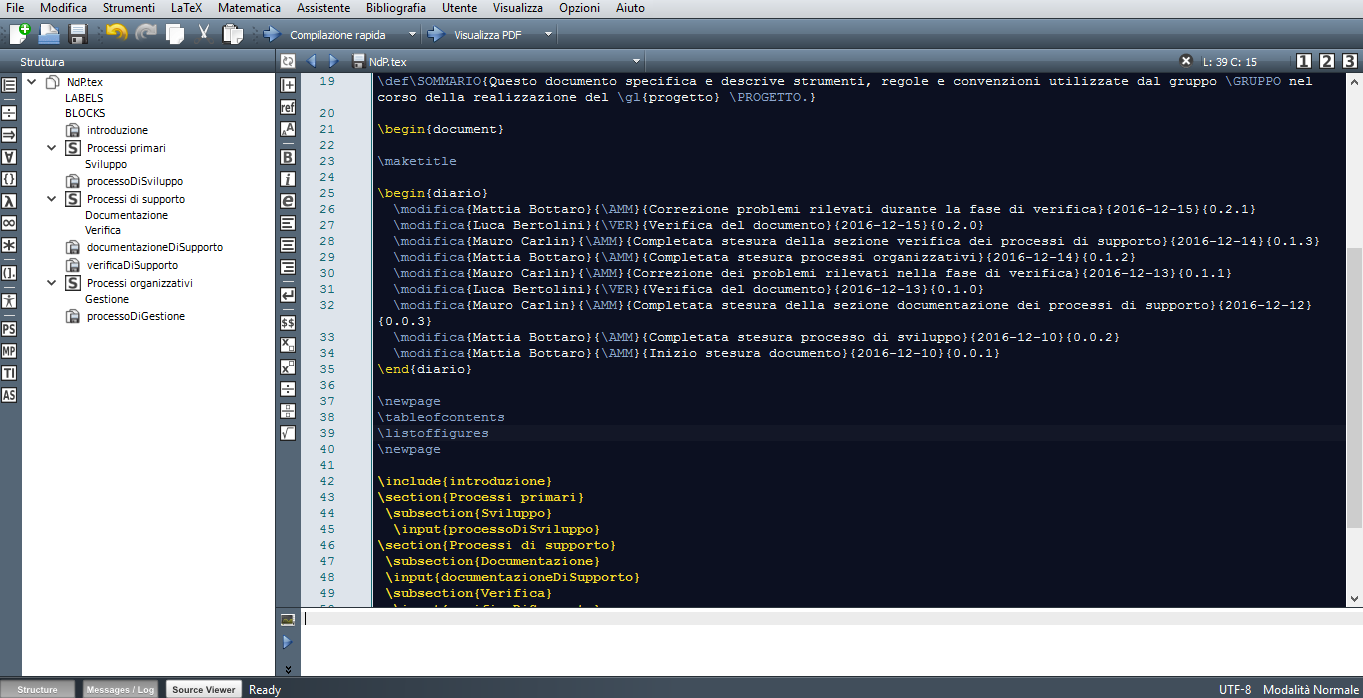
\includegraphics[scale=0.4]{img/texm.png}
\caption{Texmaker}\label{sec:Figura3}
\end{figure}
 \paragraph{Excel}
Per la creazione di grafici (istogrammi, diagrammi a torta, ecc.) viene utilizzato Excel di Microsoft Office, nella versione 2013 o successive.